\documentclass[a4paper,man,hidelinks,floatsintext]{apa7}
% This LaTeX output is designed to use APA7 style and to run on local TexLive-installation (use pdflatex) as well as on web interfaces (e.g., overleaf.com).
% To use APA6 style change apa7 to apa6 in the first line (\documentclass), comment or remove the \addORCIDlink line, and change the order of \caption and \label lines for the figures.
% If you prefer postponing your figures and table until after the reference list, instead of having them within the body of the text, please remove the ",floatsintext" from the documentclass options.
% Further information on these styles can be found here: https://www.ctan.org/pkg/apa7 and here: https://www.ctan.org/pkg/apa6

\usepackage[british]{babel}
\usepackage[utf8]{inputenc}
\usepackage{amsmath}
\usepackage{graphicx}
\usepackage[export]{adjustbox}
\usepackage{csquotes}
\usepackage[style=apa,sortcites=true,sorting=nyt,backend=biber]{biblatex}
\DeclareLanguageMapping{british}{british-apa}
\addbibresource{article.bib}

\title{APA-Style Manuscript with jamovi Results}
\shorttitle{jamovi Results}
\author{Full Name}
\leftheader{Last name}
\affiliation{Your Affilitation}
% addORCIDlink is only available from apa7
\authornote{\addORCIDlink{Your Name}{0000-0000-0000-0000}\\
More detailed information about how to contact you.\\
Can continue over several lines.
}

\abstract{Your abstract here.}
\keywords{keyword 1, keyword 2}

\begin{document}
%\maketitle

% Your introduction starts here.

%\section{Methods}
% Feel free to adjust the subsections below.

%\subsection{Participants}
% Your participants description goes here.

%\subsection{Materials}
% Your description of the experimental materials goes here.

%\subsection{Procedure}
% Your description of the experimental procedures goes here.

%\subsection{Statistical Analyses}
%Statistical analyses were performed using jamovi \parencite{jamovi}, and the R statistical language \parencite{R}, as well as the module / package GAMLj \parencite{GAMLj}.

%\section{Results}

% =========================================================================================================


<h1 contenteditable="" spellcheck="false">Results</h1>
           
      
        <p></p>
      
    
      
      
    
            <h1 contenteditable="" spellcheck="false">Mixed Model</h1>
           
      
        <p></p>
      
    
\begin{table}[!htbp]
\caption{Model Info}
\label{tab:Table_1}
\begin{adjustbox}{max size={\columnwidth}{\textheight}}
\centering
\begin{tabular}{ll}
\hline
Info                  & ~                                                                                                      \\
\hline
Estimate              & Linear mixed model fit by REML                                                                         \\
Call                  & Rating ~ 1 + Condition + Vowel + Gender + Condition:Vowel + Condition:Gender + Vowel:Gender+( 1 | ID ) \\
AIC                   & 43364.024                                                                                              \\
BIC                   & 43484.935                                                                                              \\
LogLikel.             & -21640.382                                                                                             \\
R-squared Marginal    & 0.378                                                                                                  \\
R-squared Conditional & 0.537                                                                                                  \\
Converged             & yes                                                                                                    \\
Optimizer             & bobyqa                                                                                                 \\
\hline
\end{tabular}
\end{adjustbox}
\begin{tablenotes}[para,flushleft] {
\small
}
\end{tablenotes}
\end{table}
      
        <p></p>
      
    <h2>Model Results</h2>
      
        <p></p>
      
    
\begin{table}[!htbp]
\caption{Fixed Effect Omnibus tests}
\label{tab:Table_2}
\begin{adjustbox}{max size={\columnwidth}{\textheight}}
\centering
\begin{tabular}{lrrrr}
\hline
~                           &      F & Num df & Den df &               p \\
\hline
Condition                   & 958.02 &      4 &   4896 & \textless~0.001 \\
Vowel                       &   4.60 &      2 &   4896 &           0.010 \\
Gender                      &  14.23 &      1 &   4896 & \textless~0.001 \\
Condition ~$\times$~ Vowel  &   3.47 &      8 &   4896 & \textless~0.001 \\
Condition ~$\times$~ Gender &  33.40 &      4 &   4896 & \textless~0.001 \\
Vowel ~$\times$~ Gender     &  13.86 &      2 &   4896 & \textless~0.001 \\
\hline
\end{tabular}
\end{adjustbox}
\begin{tablenotes}[para,flushleft] {
\small
\textit{Note.}~Satterthwaite method for degrees of freedom. \\
}
\end{tablenotes}
\end{table}
      
        <p></p>
      
    
\begin{table}[!htbp]
\caption{Fixed Effects Parameter Estimates}
\label{tab:Table_3}
\begin{adjustbox}{max size={\columnwidth}{\textheight}}
\centering
\begin{tabular}{llrrrrrrr}
\hline
\multicolumn{4}{c}{~} & \multicolumn{2}{c}{95\% Confidence Interval} & \multicolumn{3}{c}{~} \\
\cline{5-6}
Names                         & Effect                                             & Estimate &    SE &   Lower &   Upper &     df &       t &               p \\
\hline
(Intercept)                   & (Intercept)                                        &   59.531 & 1.959 &  55.692 &  63.369 &   32.0 &  30.396 & \textless~0.001 \\
Condition1                    & harmonic - reference                               &  -15.759 & 0.855 & -17.434 & -14.083 & 4896.0 & -18.434 & \textless~0.001 \\
Condition2                    & estimated - reference                              &  -36.639 & 0.855 & -38.315 & -34.964 & 4896.0 & -42.861 & \textless~0.001 \\
Condition3                    & synthesized - reference                            &  -41.607 & 0.855 & -43.283 & -39.932 & 4896.0 & -48.672 & \textless~0.001 \\
Condition4                    & anchor - reference                                 &  -42.458 & 0.855 & -44.133 & -40.782 & 4896.0 & -49.667 & \textless~0.001 \\
Vowel1                        & i - ( a, i, o )                                    &    0.578 & 0.382 &  -0.171 &   1.328 & 4896.0 &   1.513 &           0.130 \\
Vowel2                        & o - ( a, i, o )                                    &   -1.159 & 0.382 &  -1.908 &  -0.410 & 4896.0 &  -3.032 &           0.002 \\
Gender1                       & male - female                                      &   -2.040 & 0.541 &  -3.100 &  -0.980 & 4896.0 &  -3.773 & \textless~0.001 \\
Condition1 ~$\times$~ Vowel1  & harmonic - reference ~$\times$~ i - ( a, i, o )    &    0.995 & 1.209 &  -1.375 &   3.364 & 4896.0 &   0.823 &           0.411 \\
Condition2 ~$\times$~ Vowel1  & estimated - reference ~$\times$~ i - ( a, i, o )   &    1.497 & 1.209 &  -0.872 &   3.866 & 4896.0 &   1.238 &           0.216 \\
Condition3 ~$\times$~ Vowel1  & synthesized - reference ~$\times$~ i - ( a, i, o ) &    3.228 & 1.209 &   0.859 &   5.598 & 4896.0 &   2.670 &           0.008 \\
Condition4 ~$\times$~ Vowel1  & anchor - reference ~$\times$~ i - ( a, i, o )      &   -2.121 & 1.209 &  -4.491 &   0.248 & 4896.0 &  -1.755 &           0.079 \\
Condition1 ~$\times$~ Vowel2  & harmonic - reference ~$\times$~ o - ( a, i, o )    &   -1.963 & 1.209 &  -4.332 &   0.407 & 4896.0 &  -1.623 &           0.105 \\
Condition2 ~$\times$~ Vowel2  & estimated - reference ~$\times$~ o - ( a, i, o )   &   -2.818 & 1.209 &  -5.188 &  -0.449 & 4896.0 &  -2.331 &           0.020 \\
Condition3 ~$\times$~ Vowel2  & synthesized - reference ~$\times$~ o - ( a, i, o ) &   -2.978 & 1.209 &  -5.347 &  -0.608 & 4896.0 &  -2.463 &           0.014 \\
Condition4 ~$\times$~ Vowel2  & anchor - reference ~$\times$~ o - ( a, i, o )      &    1.094 & 1.209 &  -1.276 &   3.463 & 4896.0 &   0.905 &           0.366 \\
Condition1 ~$\times$~ Gender1 & harmonic - reference ~$\times$~ male - female      &    3.840 & 1.710 &   0.489 &   7.191 & 4896.0 &   2.246 &           0.025 \\
Condition2 ~$\times$~ Gender1 & estimated - reference ~$\times$~ male - female     &   -6.762 & 1.710 & -10.113 &  -3.411 & 4896.0 &  -3.955 & \textless~0.001 \\
Condition3 ~$\times$~ Gender1 & synthesized - reference ~$\times$~ male - female   &   -7.731 & 1.710 & -11.082 &  -4.380 & 4896.0 &  -4.522 & \textless~0.001 \\
Condition4 ~$\times$~ Gender1 & anchor - reference ~$\times$~ male - female        &    8.705 & 1.710 &   5.354 &  12.056 & 4896.0 &   5.092 & \textless~0.001 \\
Vowel1 ~$\times$~ Gender1     & i - ( a, i, o ) ~$\times$~ male - female           &   -1.710 & 0.765 &  -3.209 &  -0.212 & 4896.0 &  -2.237 &           0.025 \\
Vowel2 ~$\times$~ Gender1     & o - ( a, i, o ) ~$\times$~ male - female           &   -2.301 & 0.765 &  -3.799 &  -0.802 & 4896.0 &  -3.009 &           0.003 \\
\hline
\end{tabular}
\end{adjustbox}
\begin{tablenotes}[para,flushleft] {
\small
}
\end{tablenotes}
\end{table}
      
        <p></p>
      
    
\begin{table}[!htbp]
\caption{Random Components}
\label{tab:Table_4}
\begin{adjustbox}{max size={\columnwidth}{\textheight}}
\centering
\begin{tabular}{llrrr}
\hline
Groups   & Name        &   SD & Variance &   ICC \\
\hline
ID       & (Intercept) & 11.1 &      124 & 0.256 \\
Residual & ~           & 19.0 &      362 &     ~ \\
\hline
\end{tabular}
\end{adjustbox}
\begin{tablenotes}[para,flushleft] {
\small
\textit{Note.}~Number of Obs: 4950 , groups: ID 33. \\
}
\end{tablenotes}
\end{table}
      
        <p></p>
      
    
\begin{table}[!htbp]
\caption{Random Effect LRT}
\label{tab:Table_5}
\begin{adjustbox}{max size={\columnwidth}{\textheight}}
\centering
\begin{tabular}{lrrrrr}
\hline
Test     & N. par &   AIC &  LRT &   df &               p \\
\hline
(1 | ID) &   23.0 & 44622 & 1295 & 1.00 & \textless~0.001 \\
\hline
\end{tabular}
\end{adjustbox}
\begin{tablenotes}[para,flushleft] {
\small
}
\end{tablenotes}
\end{table}
      
        <p></p>
      
    
      
      
    
      
        <p></p>
      
    <h2>Post Hoc Tests</h2>
      
        <p></p>
      
    
\begin{table}[!htbp]
\caption{Post Hoc Comparisons - Condition}
\label{tab:Table_6}
\begin{adjustbox}{max size={\columnwidth}{\textheight}}
\centering
\begin{tabular}{lrlrrrrr}
\hline
\multicolumn{3}{c}{Comparison} & \multicolumn{5}{c}{~} \\
\cline{1-3}
Condition   & ~ & Condition   & Difference &    SE &      t &   df & p$_{bonferroni}$ \\
\hline
harmonic    & - & synthesized &     25.848 & 0.855 & 30.238 & 4896 &  \textless~0.001 \\
harmonic    & - & anchor      &     26.699 & 0.855 & 31.233 & 4896 &  \textless~0.001 \\
harmonic    & - & estimated   &     20.881 & 0.855 & 24.426 & 4896 &  \textless~0.001 \\
synthesized & - & anchor      &      0.851 & 0.855 &  0.995 & 4896 &            1.000 \\
reference   & - & harmonic    &     15.759 & 0.855 & 18.434 & 4896 &  \textless~0.001 \\
reference   & - & synthesized &     41.607 & 0.855 & 48.672 & 4896 &  \textless~0.001 \\
reference   & - & anchor      &     42.458 & 0.855 & 49.667 & 4896 &  \textless~0.001 \\
reference   & - & estimated   &     36.639 & 0.855 & 42.861 & 4896 &  \textless~0.001 \\
estimated   & - & synthesized &      4.968 & 0.855 &  5.811 & 4896 &  \textless~0.001 \\
estimated   & - & anchor      &      5.818 & 0.855 &  6.806 & 4896 &  \textless~0.001 \\
\hline
\end{tabular}
\end{adjustbox}
\begin{tablenotes}[para,flushleft] {
\small
}
\end{tablenotes}
\end{table}
      
        <p></p>
      
    
\begin{table}[!htbp]
\caption{Post Hoc Comparisons - Condition ~$\times$~ Vowel}
\label{tab:Table_7}
\begin{adjustbox}{max size={\columnwidth}{\textheight}}
\centering
\begin{tabular}{llrllrrrrr}
\hline
\multicolumn{5}{c}{Comparison} & \multicolumn{5}{c}{~} \\
\cline{1-5}
Condition   & Vowel & ~ & Condition   & Vowel & Difference &   SE &        t &   df & p$_{bonferroni}$ \\
\hline
harmonic    & i     & - & harmonic    & o     &     2.6424 & 1.48 &   1.7847 & 4896 &            1.000 \\
harmonic    & i     & - & synthesized & i     &    23.6152 & 1.48 &  15.9493 & 4896 &  \textless~0.001 \\
harmonic    & i     & - & synthesized & o     &    29.5061 & 1.48 &  19.9280 & 4896 &  \textless~0.001 \\
harmonic    & i     & - & reference   & o     &   -15.0788 & 1.48 & -10.1840 & 4896 &  \textless~0.001 \\
harmonic    & i     & - & anchor      & i     &    29.8152 & 1.48 &  20.1367 & 4896 &  \textless~0.001 \\
harmonic    & i     & - & anchor      & o     &    26.2848 & 1.48 &  17.7524 & 4896 &  \textless~0.001 \\
harmonic    & i     & - & estimated   & i     &    20.3788 & 1.48 &  13.7635 & 4896 &  \textless~0.001 \\
harmonic    & i     & - & estimated   & o     &    24.3788 & 1.48 &  16.4651 & 4896 &  \textless~0.001 \\
harmonic    & o     & - & synthesized & o     &    26.8636 & 1.48 &  18.1433 & 4896 &  \textless~0.001 \\
harmonic    & o     & - & anchor      & o     &    23.6424 & 1.48 &  15.9678 & 4896 &  \textless~0.001 \\
harmonic    & o     & - & estimated   & o     &    21.7364 & 1.48 &  14.6804 & 4896 &  \textless~0.001 \\
harmonic    & a     & - & harmonic    & i     &     0.0818 & 1.48 &   0.0553 & 4896 &            1.000 \\
harmonic    & a     & - & harmonic    & o     &     2.7242 & 1.48 &   1.8399 & 4896 &            1.000 \\
harmonic    & a     & - & synthesized & i     &    23.6970 & 1.48 &  16.0046 & 4896 &  \textless~0.001 \\
harmonic    & a     & - & synthesized & o     &    29.5879 & 1.48 &  19.9832 & 4896 &  \textless~0.001 \\
harmonic    & a     & - & synthesized & a     &    27.0667 & 1.48 &  18.2804 & 4896 &  \textless~0.001 \\
harmonic    & a     & - & reference   & i     &   -14.6818 & 1.48 &  -9.9159 & 4896 &  \textless~0.001 \\
harmonic    & a     & - & reference   & o     &   -14.9970 & 1.48 & -10.1287 & 4896 &  \textless~0.001 \\
harmonic    & a     & - & anchor      & i     &    29.8970 & 1.48 &  20.1920 & 4896 &  \textless~0.001 \\
harmonic    & a     & - & anchor      & o     &    26.3667 & 1.48 &  17.8077 & 4896 &  \textless~0.001 \\
harmonic    & a     & - & anchor      & a     &    26.6394 & 1.48 &  17.9919 & 4896 &  \textless~0.001 \\
harmonic    & a     & - & estimated   & i     &    20.4606 & 1.48 &  13.8188 & 4896 &  \textless~0.001 \\
harmonic    & a     & - & estimated   & o     &    24.4606 & 1.48 &  16.5204 & 4896 &  \textless~0.001 \\
harmonic    & a     & - & estimated   & a     &    20.5273 & 1.48 &  13.8638 & 4896 &  \textless~0.001 \\
synthesized & i     & - & harmonic    & o     &   -20.9727 & 1.48 & -14.1647 & 4896 &  \textless~0.001 \\
synthesized & i     & - & synthesized & o     &     5.8909 & 1.48 &   3.9786 & 4896 &            0.007 \\
synthesized & i     & - & reference   & o     &   -38.6939 & 1.48 & -26.1333 & 4896 &  \textless~0.001 \\
synthesized & i     & - & anchor      & i     &     6.2000 & 1.48 &   4.1874 & 4896 &            0.003 \\
synthesized & i     & - & anchor      & o     &     2.6697 & 1.48 &   1.8031 & 4896 &            1.000 \\
synthesized & i     & - & estimated   & o     &     0.7636 & 1.48 &   0.5157 & 4896 &            1.000 \\
synthesized & o     & - & anchor      & o     &    -3.2212 & 1.48 &  -2.1756 & 4896 &            1.000 \\
synthesized & a     & - & harmonic    & i     &   -26.9848 & 1.48 & -18.2252 & 4896 &  \textless~0.001 \\
synthesized & a     & - & harmonic    & o     &   -24.3424 & 1.48 & -16.4405 & 4896 &  \textless~0.001 \\
synthesized & a     & - & synthesized & i     &    -3.3697 & 1.48 &  -2.2758 & 4896 &            1.000 \\
synthesized & a     & - & synthesized & o     &     2.5212 & 1.48 &   1.7028 & 4896 &            1.000 \\
synthesized & a     & - & reference   & i     &   -41.7485 & 1.48 & -28.1963 & 4896 &  \textless~0.001 \\
synthesized & a     & - & reference   & o     &   -42.0636 & 1.48 & -28.4092 & 4896 &  \textless~0.001 \\
synthesized & a     & - & anchor      & i     &     2.8303 & 1.48 &   1.9115 & 4896 &            1.000 \\
synthesized & a     & - & anchor      & o     &    -0.7000 & 1.48 &  -0.4728 & 4896 &            1.000 \\
synthesized & a     & - & anchor      & a     &    -0.4273 & 1.48 &  -0.2886 & 4896 &            1.000 \\
synthesized & a     & - & estimated   & i     &    -6.6061 & 1.48 &  -4.4616 & 4896 &  \textless~0.001 \\
synthesized & a     & - & estimated   & o     &    -2.6061 & 1.48 &  -1.7601 & 4896 &            1.000 \\
reference   & i     & - & harmonic    & i     &    14.7636 & 1.48 &   9.9712 & 4896 &  \textless~0.001 \\
reference   & i     & - & harmonic    & o     &    17.4061 & 1.48 &  11.7558 & 4896 &  \textless~0.001 \\
reference   & i     & - & synthesized & i     &    38.3788 & 1.48 &  25.9205 & 4896 &  \textless~0.001 \\
reference   & i     & - & synthesized & o     &    44.2697 & 1.48 &  29.8991 & 4896 &  \textless~0.001 \\
reference   & i     & - & reference   & o     &    -0.3152 & 1.48 &  -0.2128 & 4896 &            1.000 \\
reference   & i     & - & anchor      & i     &    44.5788 & 1.48 &  30.1079 & 4896 &  \textless~0.001 \\
reference   & i     & - & anchor      & o     &    41.0485 & 1.48 &  27.7236 & 4896 &  \textless~0.001 \\
reference   & i     & - & estimated   & i     &    35.1424 & 1.48 &  23.7347 & 4896 &  \textless~0.001 \\
reference   & i     & - & estimated   & o     &    39.1424 & 1.48 &  26.4362 & 4896 &  \textless~0.001 \\
reference   & o     & - & harmonic    & o     &    17.7212 & 1.48 &  11.9687 & 4896 &  \textless~0.001 \\
reference   & o     & - & synthesized & o     &    44.5848 & 1.48 &  30.1120 & 4896 &  \textless~0.001 \\
reference   & o     & - & anchor      & o     &    41.3636 & 1.48 &  27.9364 & 4896 &  \textless~0.001 \\
reference   & o     & - & estimated   & o     &    39.4576 & 1.48 &  26.6491 & 4896 &  \textless~0.001 \\
reference   & a     & - & harmonic    & i     &    14.8727 & 1.48 &  10.0448 & 4896 &  \textless~0.001 \\
reference   & a     & - & harmonic    & o     &    17.5152 & 1.48 &  11.8295 & 4896 &  \textless~0.001 \\
reference   & a     & - & harmonic    & a     &    14.7909 & 1.48 &   9.9896 & 4896 &  \textless~0.001 \\
reference   & a     & - & synthesized & i     &    38.4879 & 1.48 &  25.9942 & 4896 &  \textless~0.001 \\
reference   & a     & - & synthesized & o     &    44.3788 & 1.48 &  29.9728 & 4896 &  \textless~0.001 \\
reference   & a     & - & synthesized & a     &    41.8576 & 1.48 &  28.2700 & 4896 &  \textless~0.001 \\
reference   & a     & - & reference   & i     &     0.1091 & 1.48 &   0.0737 & 4896 &            1.000 \\
reference   & a     & - & reference   & o     &    -0.2061 & 1.48 &  -0.1392 & 4896 &            1.000 \\
reference   & a     & - & anchor      & i     &    44.6879 & 1.48 &  30.1816 & 4896 &  \textless~0.001 \\
reference   & a     & - & anchor      & o     &    41.1576 & 1.48 &  27.7973 & 4896 &  \textless~0.001 \\
reference   & a     & - & anchor      & a     &    41.4303 & 1.48 &  27.9814 & 4896 &  \textless~0.001 \\
reference   & a     & - & estimated   & i     &    35.2515 & 1.48 &  23.8084 & 4896 &  \textless~0.001 \\
reference   & a     & - & estimated   & o     &    39.2515 & 1.48 &  26.5099 & 4896 &  \textless~0.001 \\
reference   & a     & - & estimated   & a     &    35.3182 & 1.48 &  23.8534 & 4896 &  \textless~0.001 \\
anchor      & i     & - & harmonic    & o     &   -27.1727 & 1.48 & -18.3521 & 4896 &  \textless~0.001 \\
anchor      & i     & - & synthesized & o     &    -0.3091 & 1.48 &  -0.2088 & 4896 &            1.000 \\
anchor      & i     & - & reference   & o     &   -44.8939 & 1.48 & -30.3207 & 4896 &  \textless~0.001 \\
anchor      & i     & - & anchor      & o     &    -3.5303 & 1.48 &  -2.3843 & 4896 &            1.000 \\
anchor      & i     & - & estimated   & o     &    -5.4364 & 1.48 &  -3.6716 & 4896 &            0.026 \\
anchor      & a     & - & harmonic    & i     &   -26.5576 & 1.48 & -17.9366 & 4896 &  \textless~0.001 \\
anchor      & a     & - & harmonic    & o     &   -23.9152 & 1.48 & -16.1520 & 4896 &  \textless~0.001 \\
anchor      & a     & - & synthesized & i     &    -2.9424 & 1.48 &  -1.9873 & 4896 &            1.000 \\
anchor      & a     & - & synthesized & o     &     2.9485 & 1.48 &   1.9914 & 4896 &            1.000 \\
anchor      & a     & - & reference   & i     &   -41.3212 & 1.48 & -27.9078 & 4896 &  \textless~0.001 \\
anchor      & a     & - & reference   & o     &   -41.6364 & 1.48 & -28.1206 & 4896 &  \textless~0.001 \\
anchor      & a     & - & anchor      & i     &     3.2576 & 1.48 &   2.2001 & 4896 &            1.000 \\
anchor      & a     & - & anchor      & o     &    -0.2727 & 1.48 &  -0.1842 & 4896 &            1.000 \\
anchor      & a     & - & estimated   & i     &    -6.1788 & 1.48 &  -4.1731 & 4896 &            0.003 \\
anchor      & a     & - & estimated   & o     &    -2.1788 & 1.48 &  -1.4715 & 4896 &            1.000 \\
estimated   & i     & - & harmonic    & o     &   -17.7364 & 1.48 & -11.9789 & 4896 &  \textless~0.001 \\
estimated   & i     & - & synthesized & i     &     3.2364 & 1.48 &   2.1858 & 4896 &            1.000 \\
estimated   & i     & - & synthesized & o     &     9.1273 & 1.48 &   6.1644 & 4896 &  \textless~0.001 \\
estimated   & i     & - & reference   & o     &   -35.4576 & 1.48 & -23.9476 & 4896 &  \textless~0.001 \\
estimated   & i     & - & anchor      & i     &     9.4364 & 1.48 &   6.3732 & 4896 &  \textless~0.001 \\
estimated   & i     & - & anchor      & o     &     5.9061 & 1.48 &   3.9889 & 4896 &            0.007 \\
estimated   & i     & - & estimated   & o     &     4.0000 & 1.48 &   2.7015 & 4896 &            0.727 \\
estimated   & o     & - & synthesized & o     &     5.1273 & 1.48 &   3.4629 & 4896 &            0.057 \\
estimated   & o     & - & anchor      & o     &     1.9061 & 1.48 &   1.2873 & 4896 &            1.000 \\
estimated   & a     & - & harmonic    & i     &   -20.4455 & 1.48 & -13.8086 & 4896 &  \textless~0.001 \\
estimated   & a     & - & harmonic    & o     &   -17.8030 & 1.48 & -12.0239 & 4896 &  \textless~0.001 \\
estimated   & a     & - & synthesized & i     &     3.1697 & 1.48 &   2.1408 & 4896 &            1.000 \\
estimated   & a     & - & synthesized & o     &     9.0606 & 1.48 &   6.1194 & 4896 &  \textless~0.001 \\
estimated   & a     & - & synthesized & a     &     6.5394 & 1.48 &   4.4166 & 4896 &            0.001 \\
estimated   & a     & - & reference   & i     &   -35.2091 & 1.48 & -23.7797 & 4896 &  \textless~0.001 \\
estimated   & a     & - & reference   & o     &   -35.5242 & 1.48 & -23.9926 & 4896 &  \textless~0.001 \\
estimated   & a     & - & anchor      & i     &     9.3697 & 1.48 &   6.3282 & 4896 &  \textless~0.001 \\
estimated   & a     & - & anchor      & o     &     5.8394 & 1.48 &   3.9438 & 4896 &            0.009 \\
estimated   & a     & - & anchor      & a     &     6.1121 & 1.48 &   4.1280 & 4896 &            0.004 \\
estimated   & a     & - & estimated   & i     &    -0.0667 & 1.48 &  -0.0450 & 4896 &            1.000 \\
estimated   & a     & - & estimated   & o     &     3.9333 & 1.48 &   2.6565 & 4896 &            0.832 \\
\hline
\end{tabular}
\end{adjustbox}
\begin{tablenotes}[para,flushleft] {
\small
}
\end{tablenotes}
\end{table}
      
        <p></p>
      
    
\begin{table}[!htbp]
\caption{Post Hoc Comparisons - Condition ~$\times$~ Gender}
\label{tab:Table_8}
\begin{adjustbox}{max size={\columnwidth}{\textheight}}
\centering
\begin{tabular}{llrllrrrrr}
\hline
\multicolumn{5}{c}{Comparison} & \multicolumn{5}{c}{~} \\
\cline{1-5}
Condition   & Gender & ~ & Condition   & Gender & Difference &   SE &       t &   df & p$_{bonferroni}$ \\
\hline
harmonic    & male   & - & synthesized & male   &     31.634 & 1.21 &  26.167 & 4896 &  \textless~0.001 \\
harmonic    & male   & - & anchor      & male   &     24.267 & 1.21 &  20.073 & 4896 &  \textless~0.001 \\
harmonic    & male   & - & estimated   & male   &     26.182 & 1.21 &  21.657 & 4896 &  \textless~0.001 \\
harmonic    & female & - & harmonic    & male   &     -2.190 & 1.21 &  -1.811 & 4896 &            1.000 \\
harmonic    & female & - & synthesized & male   &     29.444 & 1.21 &  24.356 & 4896 &  \textless~0.001 \\
harmonic    & female & - & synthesized & female &     20.063 & 1.21 &  16.595 & 4896 &  \textless~0.001 \\
harmonic    & female & - & reference   & male   &    -16.028 & 1.21 & -13.258 & 4896 &  \textless~0.001 \\
harmonic    & female & - & anchor      & male   &     22.077 & 1.21 &  18.261 & 4896 &  \textless~0.001 \\
harmonic    & female & - & anchor      & female &     29.131 & 1.21 &  24.097 & 4896 &  \textless~0.001 \\
harmonic    & female & - & estimated   & male   &     23.992 & 1.21 &  19.846 & 4896 &  \textless~0.001 \\
harmonic    & female & - & estimated   & female &     15.580 & 1.21 &  12.887 & 4896 &  \textless~0.001 \\
synthesized & male   & - & anchor      & male   &     -7.368 & 1.21 &  -6.094 & 4896 &  \textless~0.001 \\
synthesized & female & - & harmonic    & male   &    -22.253 & 1.21 & -18.407 & 4896 &  \textless~0.001 \\
synthesized & female & - & synthesized & male   &      9.382 & 1.21 &   7.760 & 4896 &  \textless~0.001 \\
synthesized & female & - & reference   & male   &    -36.091 & 1.21 & -29.854 & 4896 &  \textless~0.001 \\
synthesized & female & - & anchor      & male   &      2.014 & 1.21 &   1.666 & 4896 &            1.000 \\
synthesized & female & - & anchor      & female &      9.069 & 1.21 &   7.501 & 4896 &  \textless~0.001 \\
synthesized & female & - & estimated   & male   &      3.929 & 1.21 &   3.250 & 4896 &            0.052 \\
reference   & male   & - & harmonic    & male   &     13.838 & 1.21 &  11.447 & 4896 &  \textless~0.001 \\
reference   & male   & - & synthesized & male   &     45.473 & 1.21 &  37.614 & 4896 &  \textless~0.001 \\
reference   & male   & - & anchor      & male   &     38.105 & 1.21 &  31.520 & 4896 &  \textless~0.001 \\
reference   & male   & - & estimated   & male   &     40.020 & 1.21 &  33.104 & 4896 &  \textless~0.001 \\
reference   & female & - & harmonic    & male   &     15.489 & 1.21 &  12.812 & 4896 &  \textless~0.001 \\
reference   & female & - & harmonic    & female &     17.679 & 1.21 &  14.623 & 4896 &  \textless~0.001 \\
reference   & female & - & synthesized & male   &     47.123 & 1.21 &  38.979 & 4896 &  \textless~0.001 \\
reference   & female & - & synthesized & female &     37.741 & 1.21 &  31.219 & 4896 &  \textless~0.001 \\
reference   & female & - & reference   & male   &      1.651 & 1.21 &   1.365 & 4896 &            1.000 \\
reference   & female & - & anchor      & male   &     39.756 & 1.21 &  32.885 & 4896 &  \textless~0.001 \\
reference   & female & - & anchor      & female &     46.810 & 1.21 &  38.720 & 4896 &  \textless~0.001 \\
reference   & female & - & estimated   & male   &     41.671 & 1.21 &  34.469 & 4896 &  \textless~0.001 \\
reference   & female & - & estimated   & female &     33.259 & 1.21 &  27.511 & 4896 &  \textless~0.001 \\
anchor      & female & - & harmonic    & male   &    -31.321 & 1.21 & -25.908 & 4896 &  \textless~0.001 \\
anchor      & female & - & synthesized & male   &      0.313 & 1.21 &   0.259 & 4896 &            1.000 \\
anchor      & female & - & reference   & male   &    -45.160 & 1.21 & -37.355 & 4896 &  \textless~0.001 \\
anchor      & female & - & anchor      & male   &     -7.055 & 1.21 &  -5.835 & 4896 &  \textless~0.001 \\
anchor      & female & - & estimated   & male   &     -5.139 & 1.21 &  -4.251 & 4896 &  \textless~0.001 \\
estimated   & male   & - & synthesized & male   &      5.453 & 1.21 &   4.510 & 4896 &  \textless~0.001 \\
estimated   & male   & - & anchor      & male   &     -1.915 & 1.21 &  -1.584 & 4896 &            1.000 \\
estimated   & female & - & harmonic    & male   &    -17.770 & 1.21 & -14.699 & 4896 &  \textless~0.001 \\
estimated   & female & - & synthesized & male   &     13.865 & 1.21 &  11.468 & 4896 &  \textless~0.001 \\
estimated   & female & - & synthesized & female &      4.483 & 1.21 &   3.708 & 4896 &            0.010 \\
estimated   & female & - & reference   & male   &    -31.608 & 1.21 & -26.145 & 4896 &  \textless~0.001 \\
estimated   & female & - & anchor      & male   &      6.497 & 1.21 &   5.374 & 4896 &  \textless~0.001 \\
estimated   & female & - & anchor      & female &     13.552 & 1.21 &  11.209 & 4896 &  \textless~0.001 \\
estimated   & female & - & estimated   & male   &      8.412 & 1.21 &   6.958 & 4896 &  \textless~0.001 \\
\hline
\end{tabular}
\end{adjustbox}
\begin{tablenotes}[para,flushleft] {
\small
}
\end{tablenotes}
\end{table}
      
        <p></p>
      
    
      
      
    
      
        <p></p>
      
    <h2>Results Plots</h2>
      
        <p></p>
      
    \begin{figure}[htbp]\caption{Vowel = a}
\label{fig:Figure_1}
% (the following arrangement follows APA7; if you want to use APA6, the caption- and label-lines have to be moved to after the includegraphics-line)
\centering
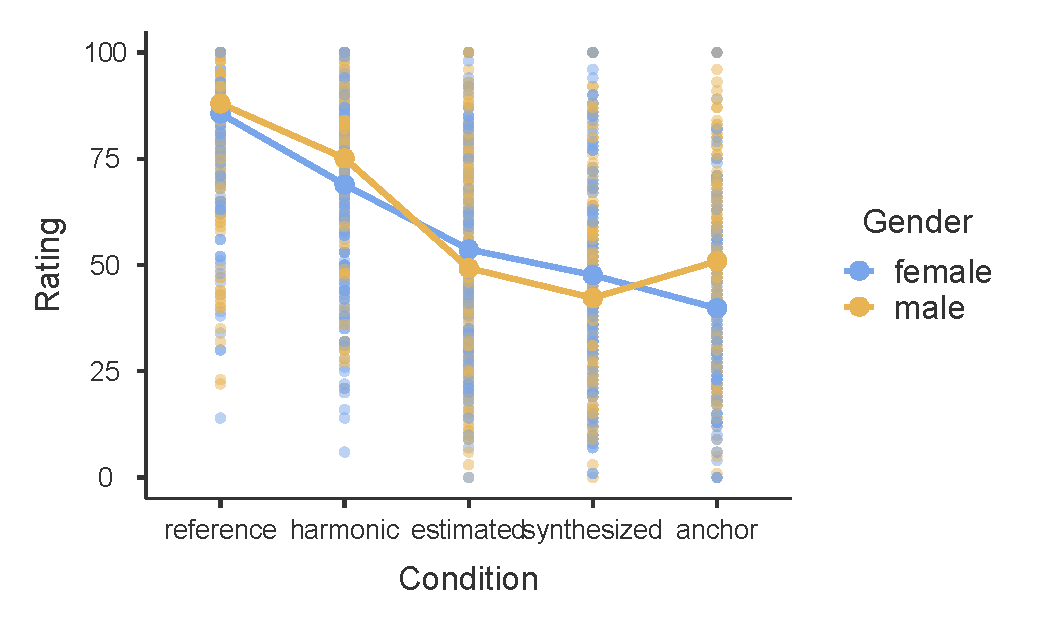
\includegraphics[width=\columnwidth]{figure_1.pdf}
\end{figure}
      
        <p></p>
      
    \begin{figure}[htbp]\caption{Vowel = i}
\label{fig:Figure_2}
% (the following arrangement follows APA7; if you want to use APA6, the caption- and label-lines have to be moved to after the includegraphics-line)
\centering
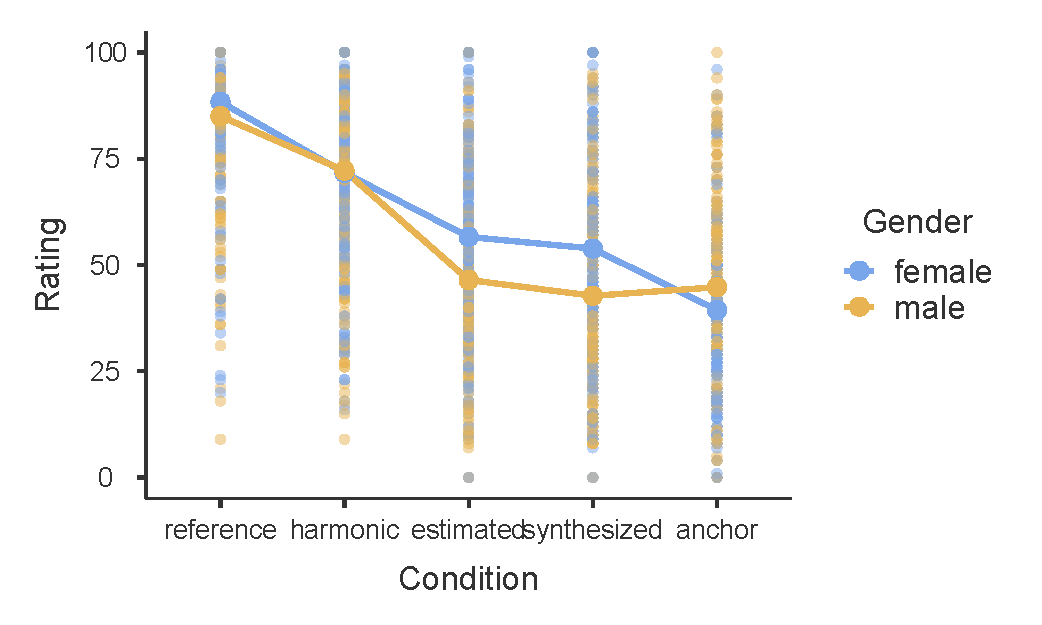
\includegraphics[width=\columnwidth]{figure_2.pdf}
\end{figure}
      
        <p></p>
      
    \begin{figure}[htbp]\caption{Vowel = o}
\label{fig:Figure_3}
% (the following arrangement follows APA7; if you want to use APA6, the caption- and label-lines have to be moved to after the includegraphics-line)
\centering
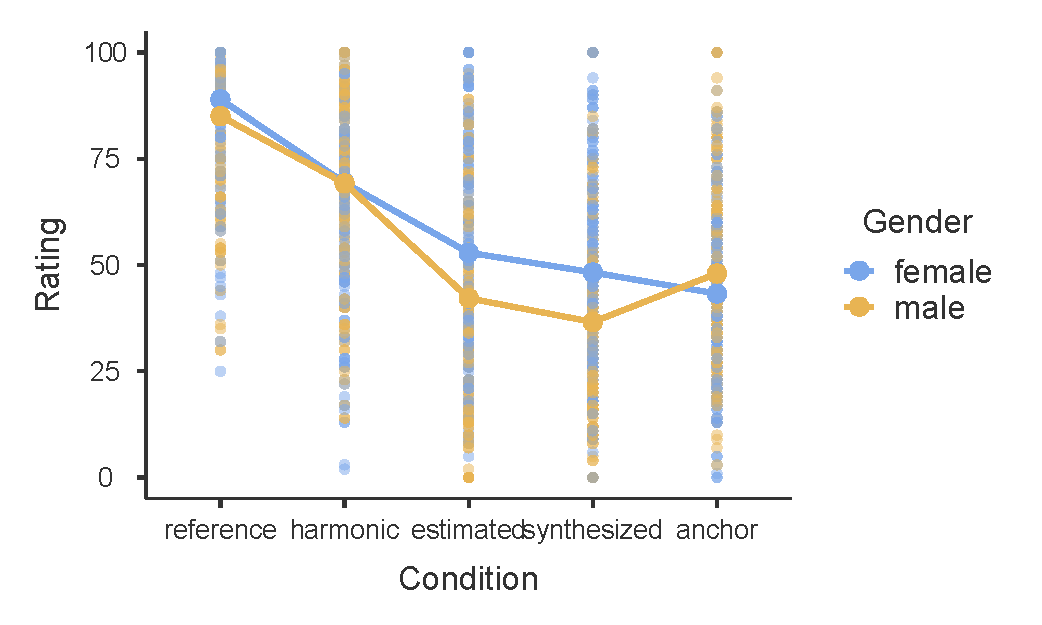
\includegraphics[width=\columnwidth]{figure_3.pdf}
\end{figure}
      
        <p></p>
      
    
      
      
    
      
        <p></p>
      
    <h2>Assumption Checks</h2>
      
        <p></p>
      
    
\begin{table}[!htbp]
\caption{Test for Normality of residuals}
\label{tab:Table_9}
\begin{adjustbox}{max size={\columnwidth}{\textheight}}
\centering
\begin{tabular}{lrr}
\hline
Test               & Statistics &               p \\
\hline
Kolmogorov-Smirnov &     0.0274 &           0.001 \\
Shapiro-Wilk       &     0.9986 & \textless~0.001 \\
\hline
\end{tabular}
\end{adjustbox}
\begin{tablenotes}[para,flushleft] {
\small
}
\end{tablenotes}
\end{table}
      
        <p></p>
      
    \begin{figure}[htbp]\caption{Residual histogram}
\label{fig:Figure_4}
% (the following arrangement follows APA7; if you want to use APA6, the caption- and label-lines have to be moved to after the includegraphics-line)
\centering

\includegraphics[width=\columnwidth]{figure_4.pdf}
\end{figure}
      
        <p></p>
      
    
      
      
    
      
        <p></p>
      
    
      
      
    
      
        <p></p>


% =========================================================================================================

% Report your results here and make references to tables (see Table~\ref{tab:Table_1}) or figures (see Figure~\ref{fig:Figure_1}).

%\section{Discussion}
% Your discussion starts here.

%\printbibliography

%\appendix

%\section{Additional tables and figures}

%Your text introducing supplementary tables and figures.

% If required copy tables and figures from the main results here.

\end{document}

